\chapter{Preprocesamiento}

\section{Acondicionamiento de la señal}

Las señales biológicas, como tantas otras, presentan contaminación en el momento de la adquisición. Éstas fuentes de
ruido, ya las mencionamos antes, provienen de ruidos respiratorios, intestinales, habla, entre otras. Por varios
motivos es recomendable realizar un pre-procesamiento de ellas para que los algoritmos que buscan características
específicas de la señal en cuestión no "se confunda". Por ejemplo, los algoritmos de delineado de \gls{ecg},
donde ubican las ondas fundamentales (P, Q, R, S, T$_{on}$, T, T$_{off}$) mejor se desempeñan cuanto más limpia o
clara es la señal. \\
\indent Un fonocardiograma presenta frecuencias entre $25-250$ Hz. Esto se debe a los sonidos fundamentales de la
señal, S$_1$ y S$_2$. El contenido espectral de S$_1$ se encuentra entre $10-180$ Hz, mientras que S$_2$ entre
$50-250$ Hz. En el primer caso, la mayor energía espectral se encuentra en componentes por debajo de los 130 Hz. Por
supuesto, que la presencia de otras frecuencias que no son intrínsecas al fonocardiograma pueden estar relacionado a
enfermedades de insuficiencia cardíaca como contaminación del entorno. \\
\indent Para realizar el filtrado se utilizaron dos filtros lineales e invariantes en el tiempo de respuesta
infinita al impulso. Un Butterworth pasa-altos y pasa-bajos. Las características de estos filtros se detallan más
adelante. Esta etapa es importante dado a que elimina ruido de contenido alto en frecuencias, que se observa un
"pasto" sobre la señal, y también remueve contenido de baja frecuencia que genera lo que se conoce como línea de
base móvil (\textit{baseline wandering}), causado por contenido de baja frecuencia como la respiración. Lo que
ocurre es que la línea isoeléctrica (\textit{baseline}) se encuentra desnivelada. Por otro lado, se remueve el valor
medio (\textit{offset}). A pesar del filtrado, algunas señales contienen ruido de baja frecuencia que no es posible
eliminar con filtros lineales, de esta forma, se aplica el algoritmo de media móvil (\textit{moving vverage}) con
una ventana de largo determinado heurísticamente para suavizar los picos. También se aplica un algoritmo de
eliminación de picos de los fonocardiogramas. Finalmente, se termina normalizando las señales para que contengan
energía unitaria. \\
\indent A continuación se observan las especificaciones de los filtros. En la Figura \ref{fig:high-pass} y
\ref{fig:low-pass} se ilustran las magnitudes de los filtros y las fases, y en la Figura \ref{fig:high-pass-tb} y
\ref{fig:low-pass-tb} las bandas de transición.

\begin{table}[H]
  \centering
  \begin{tabularx}{\textwidth}{|X|l|l|l|l|l|l|}
    \hline
    \textbf{Filtro} & \textbf{Orden} & \textbf{A}$_+$ & \textbf{A}$_-$ & $\omega_c$ & $\omega_+$ & $\omega_-$  \\
    \hline
    \thead{Pasa-altos} & \thead{4} & \thead{0.01} & \thead{0.01} & \thead{25 Hz} & \thead{41 Hz} & \thead{1.5 Hz} \\
    \hline
    \thead{Pasa-bajos} & \thead{4} & \thead{0.01} & \thead{0.01} & \thead{400 Hz} & \thead{467 Hz} & \thead{345 Hz} \\
    \hline

  \end{tabularx}

  \caption[Tabla de especificaciones de los filtros]{Tabla de especificaciones de los filtros. A$_+$ es la atenuación
  de la banda de paso, \textbf{A}$_-$ la atenuación de la banda de rechazo, $\omega_c$ la frecuencia de corte,
  $\omega_+$ la frecuencia de paso y $\omega_-$ la frecuencia de rechazo.}

\end{table}

\pagebreak

\begin{figure}[H]
  \centering
  \begin{subfigure}[b]{\textwidth}
    \centering
    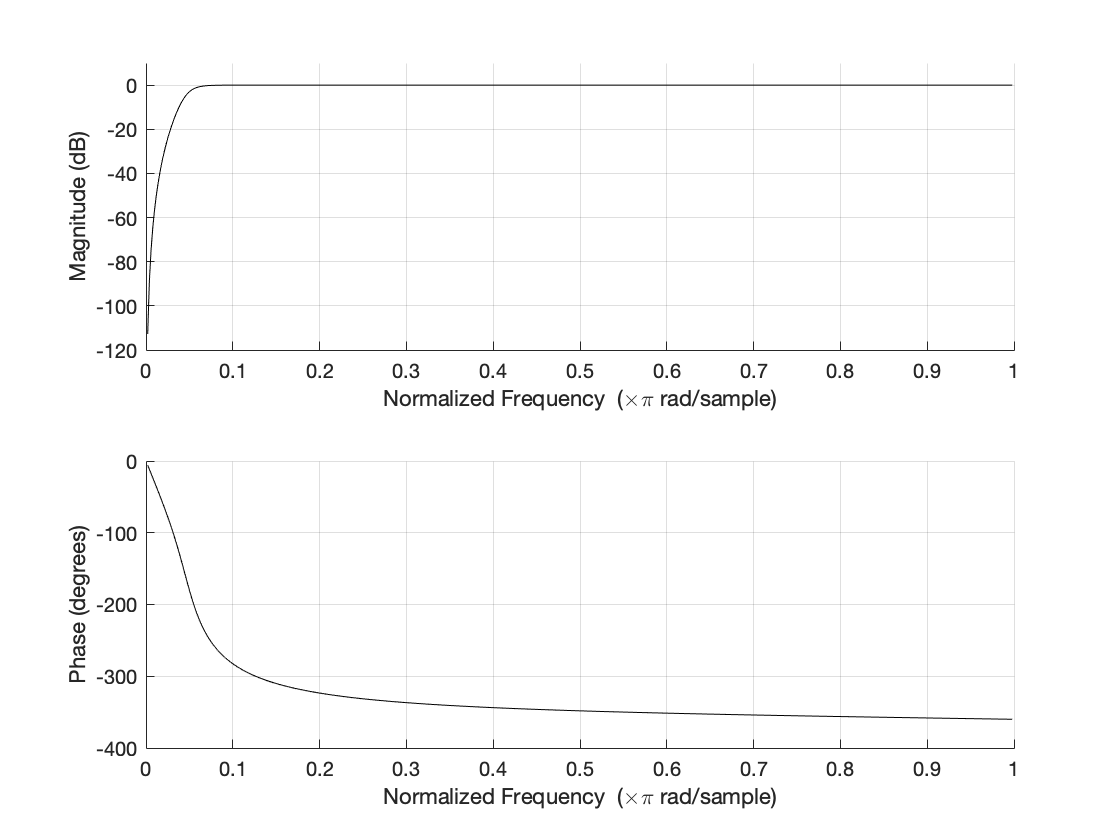
\includegraphics[scale=0.35]{sections/chapter-04/images/high-pass.png}
    \caption[Magintud y fase del filtro pasa-altos]{Magintud y fase del filtro pasa-altos.}
    \label{fig:high-pass}
  \end{subfigure} \\
  \begin{subfigure}[b]{\textwidth}
    \centering
    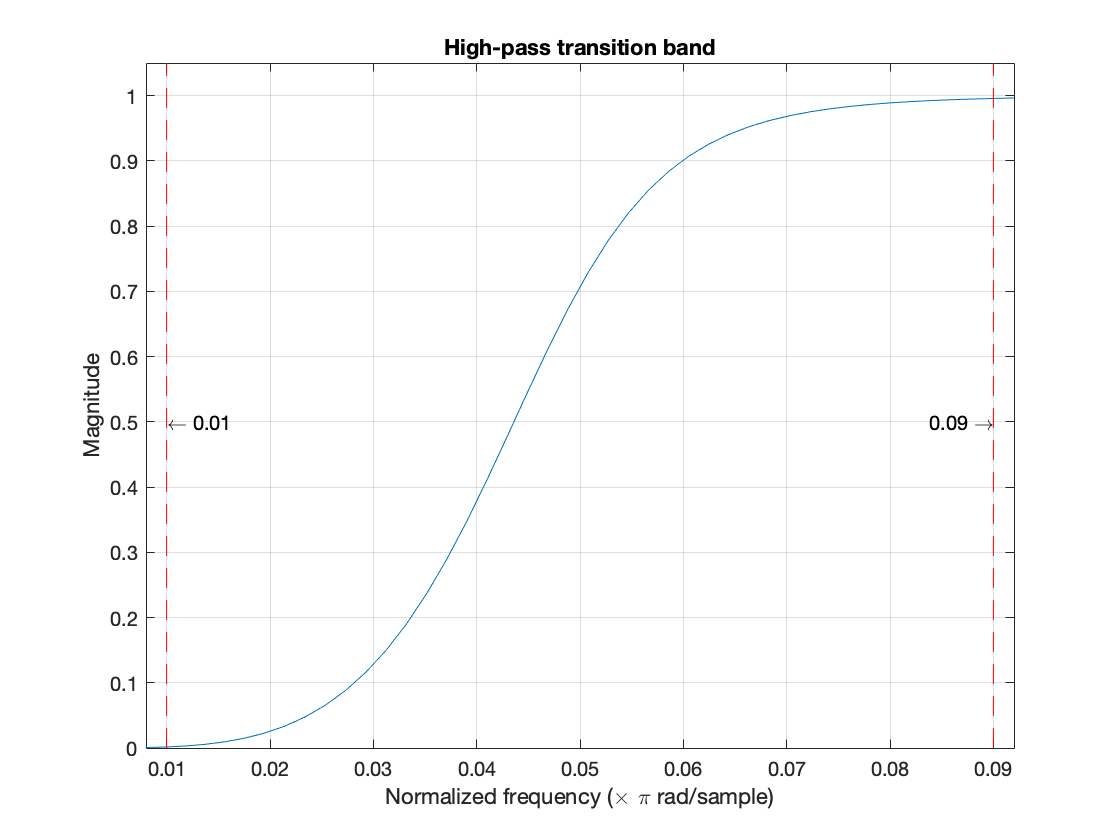
\includegraphics[scale=0.35]{sections/chapter-04/images/high-pass-tb.png}
    \caption[Banda de transición del filtro pasa-altos]{Banda de transición del filtro pasa-altos.}
    \label{fig:high-pass-tb}
  \end{subfigure}
  \caption[Filtro pasa-altos]{Filtro pasa-altos.}
\end{figure}

\begin{figure}[H]
  \centering
  \begin{subfigure}[b]{\textwidth}
    \centering
    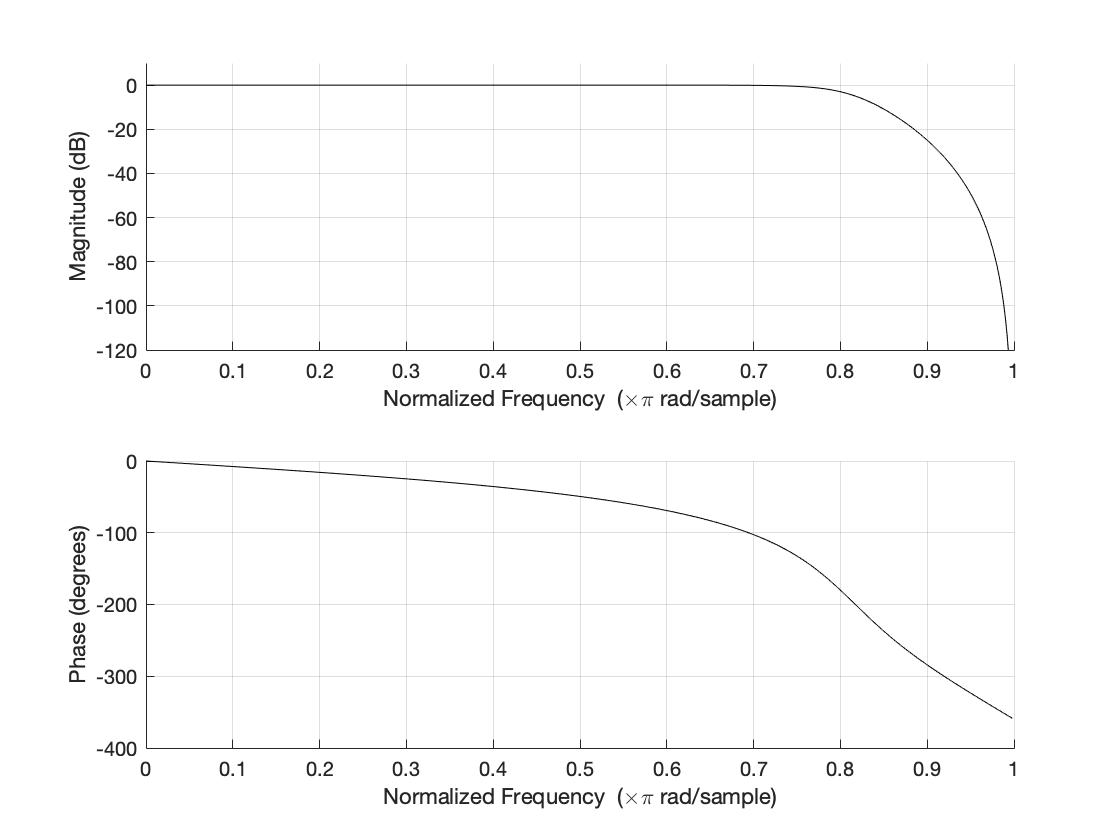
\includegraphics[scale=0.35]{sections/chapter-04/images/low-pass.png}
    \caption[Magintud y fase del filtro pasa-bajos]{Magintud y fase del filtro pasa-bajos.}
    \label{fig:low-pass}
  \end{subfigure} \\
  \begin{subfigure}[b]{\textwidth}
    \centering
    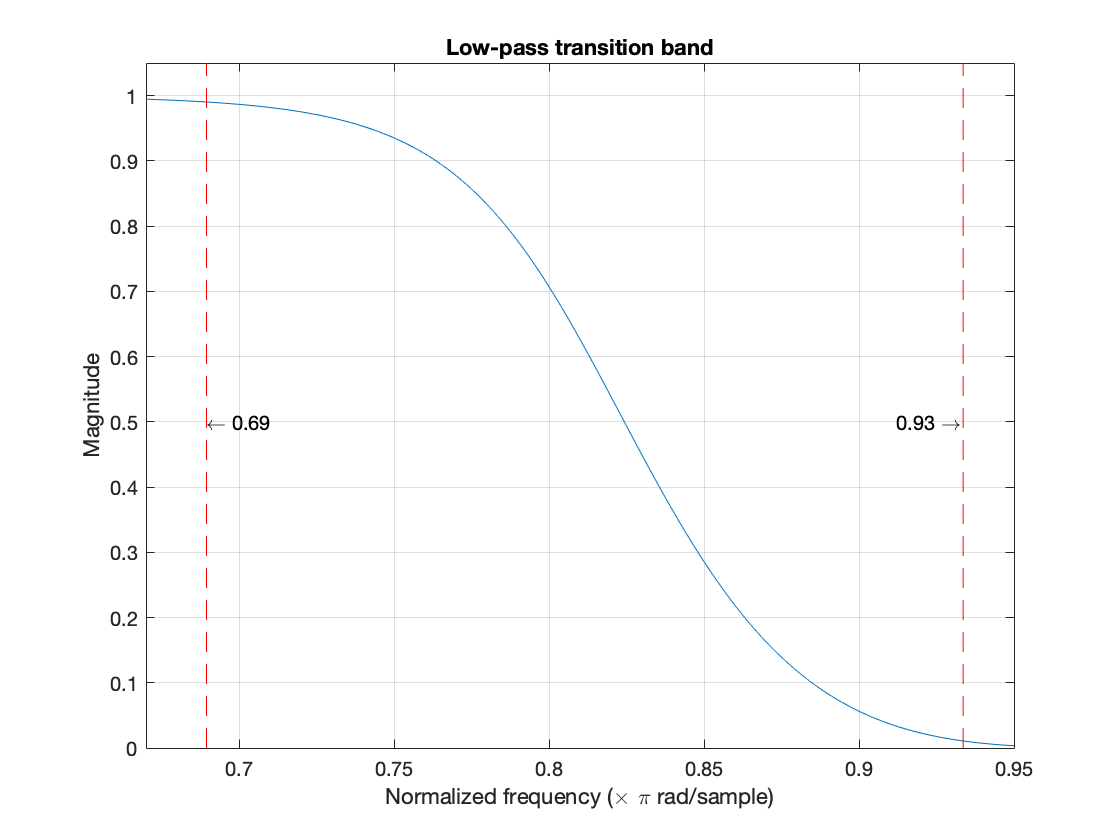
\includegraphics[scale=0.35]{sections/chapter-04/images/low-pass-tb.png}
    \caption[Banda de transición del filtro pasa-bajos]{Banda de transición del filtro pasa-bajos.}
    \label{fig:low-pass-tb}
  \end{subfigure}
  \caption[Filtro pasa-bajos]{Filtro pasa-bajos.}
\end{figure}

\pagebreak

\subsubsection*{Eliminación de picos de fricción}

\indent Los picos de fricción deben ser eliminados dado que estos picos generalmente pueden tener mayor amplitud que
los sonidos fundamentales del fonocardiograma. A continuación se presenta el algoritmo para realizar dicho
procesamiento. \bigskip

\indent Dada una señal de fonocardiograma $\bm{x}_i \in \mathbb{R}^N$ muestreada a una frecuencia de muestreo $F_s$,
se elige una ventana de largo arbitrario, i.e. $L = \left[\frac{F_s}{2}\right]$. \bigskip

\indent La idea fundamental es dividir el \gls{pcg} en ventanas de longitud $L$. Debido a esto si el módulo
entre la longitud de la señal y el largo de la ventana definido no es cero, algunas muestras quedarán fuera de
alguna de las ventanas. Estas muestras se denominan muestras residuales que no participan en el algoritmo y deben
ser agregadas al final para recuperar la señal. El número de muestras residuales se definen en la siguiente ecuación.

\begin{align}
  r_s = \mathrm{mod}(N,L)
\end{align}

\indent Definimos la ventana $\bm{w}_i \in \mathbb{R}^L$, con $i = 0,1,\dots,\left\lfloor \frac{N}{L} \right\rfloor$
. Luego, definimos al vector de los máximos, $\bm{m} \in \mathbb{R}^{\left\lfloor \frac{N}{L} \right\rfloor}$. Este
vector contiene los valores máximos de las ventanas, denominados \textit{Maximum Absolute Amplitude} (\gls{maa}).

\begin{align}
  m_i = \mathrm{max} \; \bm{w}_i
\end{align}

\indent Las componentes $m_i$ dinámicamente irán cambiando de valor hasta que ninguna de ellas sea superior a 3
veces la mediana de $\bm{m}$. Esta es la condición donde el algoritmo reconstruye la señal filtrada. \bigskip

\indent Hasta que no se cumpla la condición antes mencionada, se busca entre las ventanas la que contenga el mayor
pico.

\begin{align}
  i_{\bm{w}} = \arg \underset{i}{\mathrm{max}} (\bm{m})
\end{align}

\indent Una vez hecho esto es necesario encontrar la posición del pico en la ventana asociada.

\begin{align}
  i_{spike} = \arg \underset{i}{\mathrm{max}} (\bm{w}_{i_{\bm{w}}})
\end{align}

\indent El índice $i_{spike}$ hace referencia al valor máximo del pico de fricción. Sin embargo, es necesario
computar el comienzo y el fin del pico para eliminarlo. Para ello se necesitan computar los cruces por cero.

\begin{align}
  s_i = sgn(w_i)
\end{align}

\indent Donde $s_i$ son las componentes del vector que $\mathbf{s}_i \in \mathbb{R}^L$. Luego, se computan los
cruces por cero, $\mathbf{z} \in \mathbb{R}^{L-1}$ en la ecuación \ref{eq:zero-crossings}

\begin{align} \label{eq:zero-crossings}
z_i = s_i - s_{i-1}, \quad 0 \leq i \leq L-2
\end{align}

\indent A partir de este momento sólo queda definir el inicio y el fin del pico. El inicio del pico se encuentra a
partir del último cruce por cero hasta la posición $i_{spike}$. El final del pico, se encuentra con el primero cruce
por cero despuées de $i_{spike}$. Las ecuaciones \ref{eq:spike-start} y \ref{eq:spike-end} reflejan el cálculo.

\begin{align} \label{eq:spike-start}
p = \mathrm{max}\big\{n \in \mathbb{N}_0 \; | \; n \leq i_{spike}-1\big\}
\end{align}

\begin{align} \label{eq:spike-end}
q = \mathrm{min}\big\{n \in \mathbb{N}_0 \; | \; i_{spike} \leq n \leq L-2\big\}
\end{align}

\indent Es posible que el vector de cruces por cero sea nulo, con lo cual los valores de $p$,$q$ deberían coincidir
con el primer índice de la ventana y el último respectivamente. Luego, simplemente queda por eliminar este pico.

\begin{align}
  w_{i,j} = \epsilon, \quad p \leq j \leq q
\end{align}

\indent Siendo $\epsilon$ un número tan chico como sea defina. Por último, queda por recalcular el vector
$\mathbf{m}$ con $\mathbf{w}_i$ actualizado. \bigskip

\indent Cuando se cumpla la condición de 3 veces la mediana de $\mathbf{m}$, se concatenan todas las ventanas y se
agregan al final las muestras residuales. \bigskip

\subsubsection*{Suavizador - Media móvil}

\indent En la Figura \ref{fig:springer-pcg-example} se ilustra un fonocardiograma de un paciente sano en donde se ve
que presenta ciertas oscilaciones, luego de ser filtrado por los filtros lineales anteriores. \\
\indent Mediante un algoritmo suavizador, se aplica un ventaneo de media móvil, donde se desliza la ventana a lo
largo de toda la señal calculando el promedio de cada una de las muestras. Además, se encuentra aplicado el
algoritmo de remoción de picos de los \gls{pcg}.

\begin{figure}[H]
  \centering
  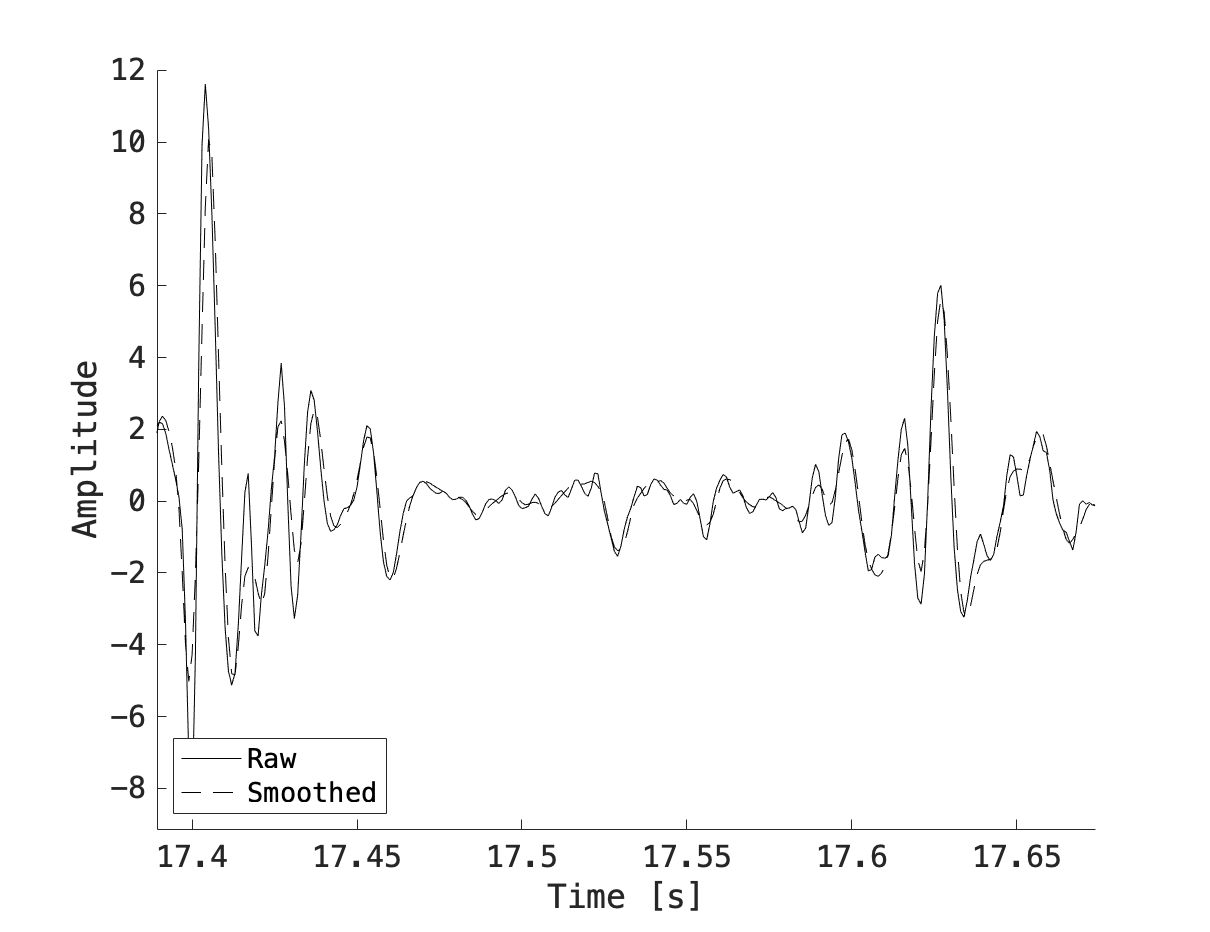
\includegraphics[scale=0.3]{sections/chapter-07/images/pcg-example.png}
  \caption[Segmento del fonocardiograma de un paciente sano]{Segmento del fonocardiograma de un paciente sano. En
  línea sólida se muestra la entrada sin ningún tipo de acondicionamiento y en línea punteada la señal suavizada.}
  \label{fig:springer-pcg-example}
\end{figure}

\section{Extracción de marcas} \label{sec:annotations}

\indent El etiquetamiento de los fonocardiogramas de entrenamiento necesitan de las anotaciones de la onda R y del
fin de la onda T. Esto fue propuesto por Schmidt \textit{et al.} en \cite{pp:schmidt2010}, donde propone que los
sonidos fundamentales del fonocardiograma, S$_1$ y S$_2$ tienen una media y un desvío asociado. Simplemente midió la
duración de S$_1$ y S$_2$ para luego calcular la media y el desvío muestral, concluyendo que la duración se mantiene
relativamente constante siendo de ($122 \pm 32$) ms y ($92 \pm 28$) ms con un $95\%$ de intervalo de confianza. \\
\indent Para la extracción de marcas del \gls{ecg}, éstas fueron hechas automáticamente por algoritmos de
delineación. Para ello se compararon 4 detectores para la detección de la onda R y el fin de la onda T. El hecho de
que haya ruido y artefactos en el \gls{ecg} provocará que las anotaciones de los detectores no coincidan. Para
ello, para asegurar que las anotaciones sean de calidad, se derivó un \textit{Signal Quality Index} (SQI) mediante
la concordancia entre los detectores. \\
\indent Los detectores utilizados para la detección de la onda R fueron gQRS, jQRS (anteriormente utilizados en
\cite{ref:behar} y \cite{ref:behar-oster-clifford}), el algoritmo basado en lo que se conoce como \textit{Parabolic
fitting} utilizado en \cite{ref:illanes-zhang} y el delineador de onditas. Ahora para la detección del fin de la
onda T se utilizó el algoritmo conocido como \textit{ecgpuwave} (basado en la detección previa del complejo QRS), un
método basado en maximizar el área de una ventana móvil entre sucesivas ondas R \cite{ref:zhang}, el delineador de
onditas y un algoritmo hecho por Vazquez-Seisdedos et al. \cite{ref:seisdedos}. Para decir que los detectores son
consistentes entre si las anotaciones no deben estar más alejadas que 100 ms.

\begin{figure}[H]
  \centering
  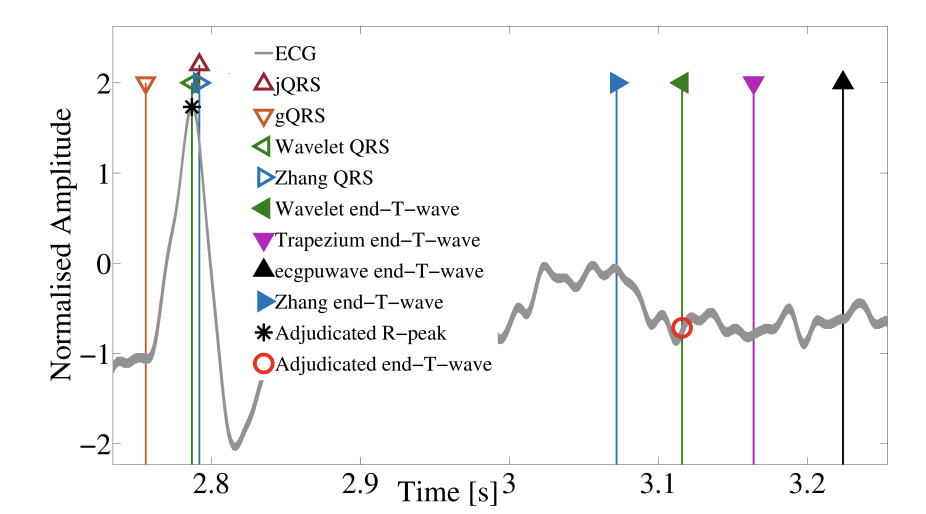
\includegraphics[scale=0.8]{sections/chapter-04/images/detector-agreement.png}
  \caption[Ejemplo de las anotaciones de una señal de \gls{ecg} con ruido. La posición de las anotaciones
  para cada uno de los detectores se muestran]{Ejemplo de las anotaciones de una señal de \gls{ecg} con ruido
  . La posición de las anotaciones para cada uno de los detectores se muestran. Imagen extraída de
  \cite{pp:springer2015}.}
  \label{fig:detector-agreement}
\end{figure}

\section{Etiquetamiento}

\indent El etiquetamiento (\textit{labeling}), corresponde a obtener etiquetas realizadas de forma manual o
automática generalmente utilizadas en el entrenamiento del modelo propuesto. Este método es lo que se conoce como
\textit{aprendizaje supervisado}, donde se necesita tener catalogada la entrada para estimar los parámetros del
modelo. \\
\indent El etiquetamiento, como se ha explicado en el Sección \ref{sec:annotations}, consiste en estimar los tiempos
de duración de los sonidos. Sin embargo, para el conjunto de datos de este trabajo, las estimaciones de Schmidt
\textit{et. al} no dieron buenos resultados, dado a que en el momento del etiquetamiento los estados no quedaban
bien definidos. Para ello, se modificaron las medias a ($122 \pm 22$) ms y ($152 \pm 22$) ms. Es necesario mencionar
que el algoritmo propuesto por Springer \textit{et. al} sea, tal vez, el responsable de la necesidad de adaptar los
parámetros de manera ad hoc. \\
\indent En la Figura \ref{fig:pcg-labeling} se observa una porción de una señal de \gls{pcg} donde, en base a
las marcas proveídas por la base de datos, se realiza el etiquetado de los estados de la señal [sístole (S$_1$),
sístole isovolumético, diástole (S$_2$), diástole isovolumétrico].

\begin{figure}[H]
  \centering
  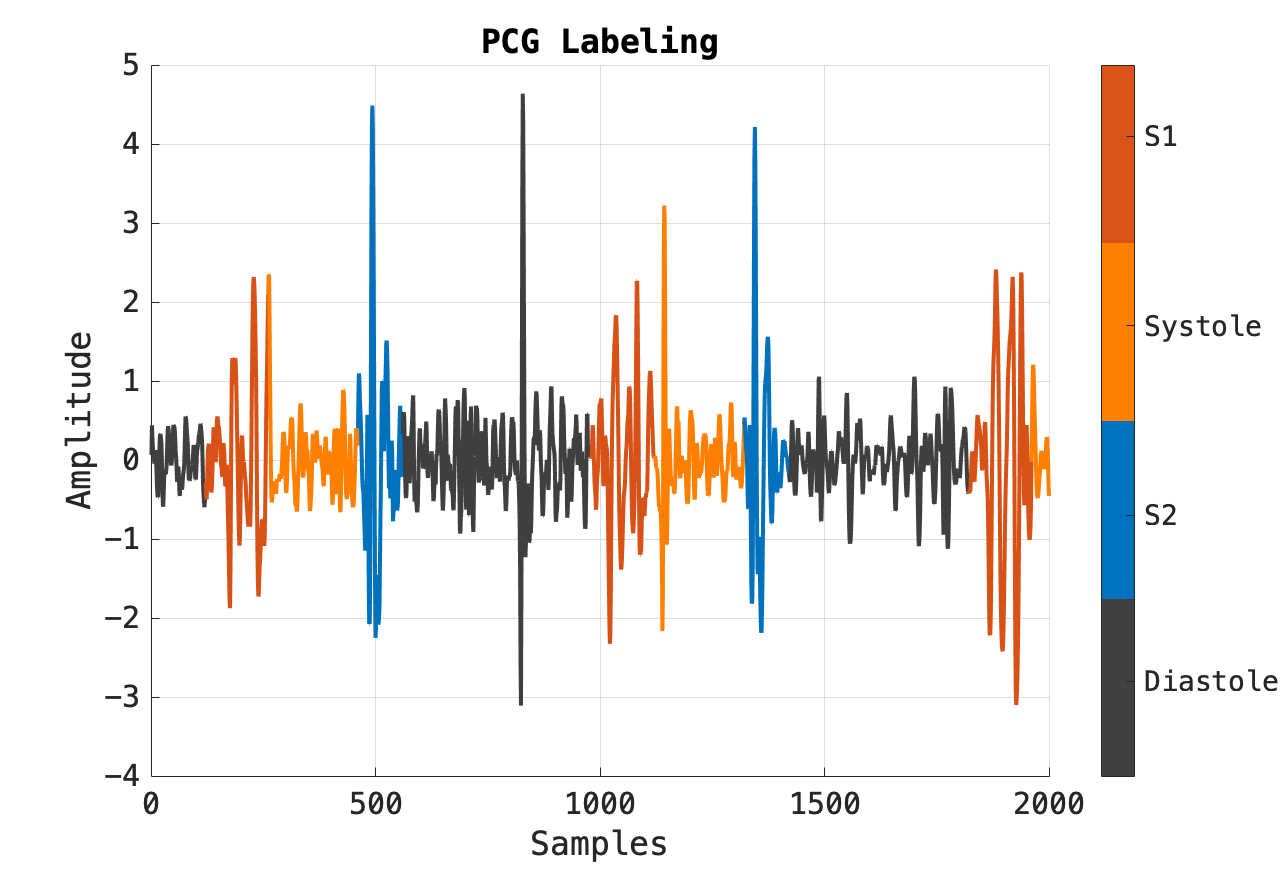
\includegraphics[scale=0.3]{sections/chapter-04/images/pcg-labeling.png}
  \caption[Segmento de una señal de fonocardiograma etiquetada]{Segmento de una señal de fonocardiograma
  etiquetada. En color rojo se marcan los sonidos S$_1$, en naranja el sístole isovolumétrico, en azul los sonidos
  S$_2$ y en negro el diástole isovolumétrico.}
  \label{fig:pcg-labeling}
\end{figure}

\subsection*{Algoritmo etiquetador}

\indent Sea una señal envolvente del fonocardiograma $\bm{x}_i \in \mathbb{R}^{N_i}$ y las posiciones de las marcas
del electrocardiograma asociadas $\bm{r}_i \in \mathbb{R}^{M_i}$, $\mathbf{t}_i \in \mathbb{R}^{M_i}$. Se definen
las medias y desvíos de los sonidos, ($\mu_{S_1}, \sigma_{S_1}$) y ($\mu_{S_2}, \sigma_{S_2}$). \bigskip

\indent Se define $\mathbf{s}_i \in \mathbb{R}^{N_i}$ al vector de estados de la señal. Recordar que este vector
sólo puede tomar 4 valores, $\mathbf{s}_i \in [1,4]$. \\
\indent A partir de aquí se mencionara el algoritmo para etiquetar cada uno de los cuatro estados.

\subsubsection*{Primer sonido (Estado \#1)}

\indent Para el marcado del primer sonido o estado, se define un umbral superior en base a la posición de la onda R.

\begin{align}
  U_{b,i} = \left[\mathrm{min}(N_i,\mathbf{r}_i+\mu_{S_1})\right]
\end{align}

\indent Donde $[x]$ es el entero más cercano a $x$.

\begin{align}
  \bm{s}_j = \mathds{1}\left\{\mathrm{max}(1, \mathbf{r}_i) < j < \mathrm{min}(U_{b,i}, N_i)\right\}
\end{align}

\subsubsection*{Segundo sonido (Estado \#3)}

\indent Para el etiquetado del segundo sonido o tercer estado, se requiere definir una ventana de búsqueda como así
también dos umbrales, uno inferior y otro superior. \\
\indent Los umbrales se definen de la siguiente manera y dependen de cada una de los finales de las ondas T.

\begin{align}
  U_{b,i} = \mathrm{min}(N_i,\lceil t_i+\lfloor \mu_{S_2} + \sigma_{S_2} \rfloor \rceil)
\end{align}

\begin{align}
  L_{b,i} = \mathrm{max}(t_i-\lfloor \mu_{S_2} + \sigma_{S_2} \rfloor,1)
\end{align}

\indent Se define los enteros superiores e inferiores según la siguiente notación.

\begin{align*}
  \lceil x \rceil := \mathrm{sup}\big\{n \; | \; n \in \mathbb{Z}, \hspace{2mm} x \leq n\big\} \\
  \lfloor x \rfloor := \mathrm{inf}\big\{n \; | \; n \in \mathbb{Z}, \hspace{2mm} x \geq n\big\}
\end{align*}

\indent Luego, se define la ventana de búsqueda en la ecuación \ref{eq:search-window}. Para cada posición del final
de la onda T se define una ventana. En ella se busca el índice del máximo valor.

\begin{align}
  \label{eq:search-window}
  \bm{\Tilde{s}}_{w,i} = \prod_{k=L_{b,i}}^{U_{b,i}} \bm{x}_k \cdot \mathds{1}\big\{\mathbf{s}_k \neq 1\big\}
\end{align}

\begin{align}
  l_i = \arg \underset{j \in [L_{b,i},U_{b,i}]}{\mathrm{max}} \Big(\bm{\Tilde{s}}_{w,i}\Big)
\end{align}

\indent Una vez extraído la posición del máximo, es necesario calcular el centro de la ventana.

\begin{align}
  c_{w,i} = \mathrm{min}\Big(N_i,l_i+L_{b,i}\Big)
\end{align}

\subsubsection*{Diástole isovolumétrico (Estado \#4)}

\indent De esta manera es posible calcular las muestras que corresponden al tercer estado. Antes es necesario
redefinir el umbral superior.

\begin{align}
  U_{b,i} = \mathrm{min}\left(N_i, \left\lceil  c_{w,i} + \frac{1}{2}\mu_{S_2} \right\rceil \right)
\end{align}

\begin{align}
  \mathbf{s}_j = 3 \cdot \mathds{1}\left\{\mathrm{max}\left(\lceil c_{w,i}-\frac{1}{2}\mu_{S_2}\rceil, 1\right) < j
  < U_{b,i}\right\}
\end{align}

\indent Con $j=0,1,2,\dots,M-1$. \bigskip

\indent Una vez definidos los estados 1 y 3, correspondientes a S$_1$ y S$_2$ respectivamente, es posible definir el
cuarto estado. \\
\indent Es necesario obtener la diferencia entre todos las posiciones de la onda R y la onda T. Para ello se define
el vector $\mathbf{d}_i \in \mathbb{R}^M$, donde sus componentes son $d_{j,i}$, con $i = 0,1,2,\dots,M-1$ y $j = 0,
1,2,\dots,M-1$.

\begin{align}
  d_{j,i} = \begin{cases}
    \infty, \qquad &r_j - t_i < 0 \\
    r_j - t_i, \quad &\mathrm{otro \; caso}
  \end{cases}
\end{align}


\begin{align}
  p_i = \begin{cases}
    N, \quad &\sum_{j=1}^{M_i} \mathds{1}\big\{d_{j,i} < \infty\big\} =  0  \\
    t_{\arg \underset{j}{\mathrm{min}} \; \mathbf{d}_i} -1, \quad  & \mathrm{otro \; caso}
  \end{cases}
\end{align}

\begin{align}
  \mathbf{s}_j = 4 \cdot \mathds{1}\left\{\left\lceil c_{w,i} + \frac{1}{2}(\mu_{S_2} + \sigma_{S_2}) \right\rceil <
  j < p_i  \right\}
\end{align}

\subsubsection*{Inicio y fin de la señal}

\indent Dado a que todos los estados derivan de la posición de la onda R y del fin de la onda T, el primer estado en
la señal siempre será 1 o 3. Por lo tanto, hasta ese estado, debe ser 2 o 4 respectivamente.

\indent Tanto para el inicio como el fin de la señal es necesario obtener desde izquierda a derecha la posición del
primer estado y el último estado en $\mathbf{s}$. Las ecuaciones \ref{eq:min-index}, \ref{eq:max-index} reflejan
como calcular dichos índices.

\begin{align} \label{eq:min-index}
  f_n = \mathrm{min}\big\{ n \in \mathbb{N}_0, \; | \; s_n \neq 0  \big\}
\end{align}

\begin{align} \label{eq:max-index}
  l_n = \mathrm{max}\big\{ n \in \mathbb{N}_0, \; | \; s_n \neq 0  \big\}
\end{align}

\indent Luego, se definen los estados del inicio y del final de la señal.

\begin{align}
  s_j = \begin{cases}
    2, \quad s_{f_n} = 3  \\
    4, \quad s_{f_n} = 1
  \end{cases}, \quad \mathrm{con} \; j = 0,1,\dots,f_n-1
\end{align}

\begin{align}
  s_j = \begin{cases}
    2, \quad s_{l_n} = 1  \\
    4, \quad s_{l_n} = 3
  \end{cases}, \quad \mathrm{con} \; j = l_n+1,l_n+2,\dots,M-1
\end{align}

\subsubsection*{Sístole isvolumétrico (Estado \#2)}

\indent Todos los estados las muestras que no han sido definidos son las correspondientes al estado 2.

\begin{align}
  s_j = \begin{cases}
    2, \quad s_j = 0  \\
    s_j, \quad s_j \neq 0
  \end{cases}, \quad \mathrm{con} \; j = 0,1,\dots,M-1
\end{align}
